\documentclass[usenames,dvipsnames]{beamer}
\usepackage[utf8]{inputenc}
\usepackage{xfrac}
\usepackage{amsmath}
\usepackage{graphicx}
\usepackage{dsfont}
\usepackage{apacite}
\usepackage{adjustbox}
\usepackage{booktabs}
\usepackage{amsfonts}
\usepackage{hyperref}
\usepackage{pdflscape}
\usepackage{lscape}
\usepackage{caption}
\usepackage{subcaption}
\usepackage{pgfplots}
\usepackage{xcolor}
\usepackage{epstopdf}
\usepackage{euler}
\usepackage{bbm}
\usepackage{multicol}
\usepackage{ulem}
\usepackage{cancel}
\usepackage{bbm}



\hypersetup{
    colorlinks,%
    citecolor=black,%
    filecolor=black,%
    linkcolor=black,%
    urlcolor=black
}   % useful for program listings
\usepackage{natbib}
\usecolortheme{seahorse}

\title{Metodología para calcular de la Contraprestación Adicional en títulos Mineros }
\author{Jose M. Quintero}
\date{May 26, 2021}

% Delete this, if you do not want the table of contents to pop up at
% the beginning of each subsection:

\AtBeginSection[]
{
  \begin{frame}<beamer>
    \frametitle{Outline}
    \tableofcontents[currentsection]
  \end{frame}
}


\begin{document}

\begin{frame}
  \titlepage
\end{frame}

\begin{frame}{Propuesta Actual}
\begin{itemize}
    \item La propuesta actual usa la fórmula
    \begin{equation*}
        Ca = X\times Po\times Pa\%
    \end{equation*}
    donde 
    \begin{enumerate}
        \item $X$ representa la cantidad total de mineral producido y tipo de mineral (térmico o metalúrgico), 
        \item $Po$ representa el precio base de liquidación de regalías fijado por la UPME del trimestre en liquidación, y 
        \item $Pa\%$ corresponde a la participación (porcentaje) ofrecida por el Contratista. 
    \end{enumerate}
    \item El cálculo actual de $Pa$ no explota el hecho que la evolución de los precios tiene una estructura. 
\end{itemize}
\end{frame}

\begin{frame}{Precios Base Regalia}{Térmico}
    \begin{figure}
        \centering
        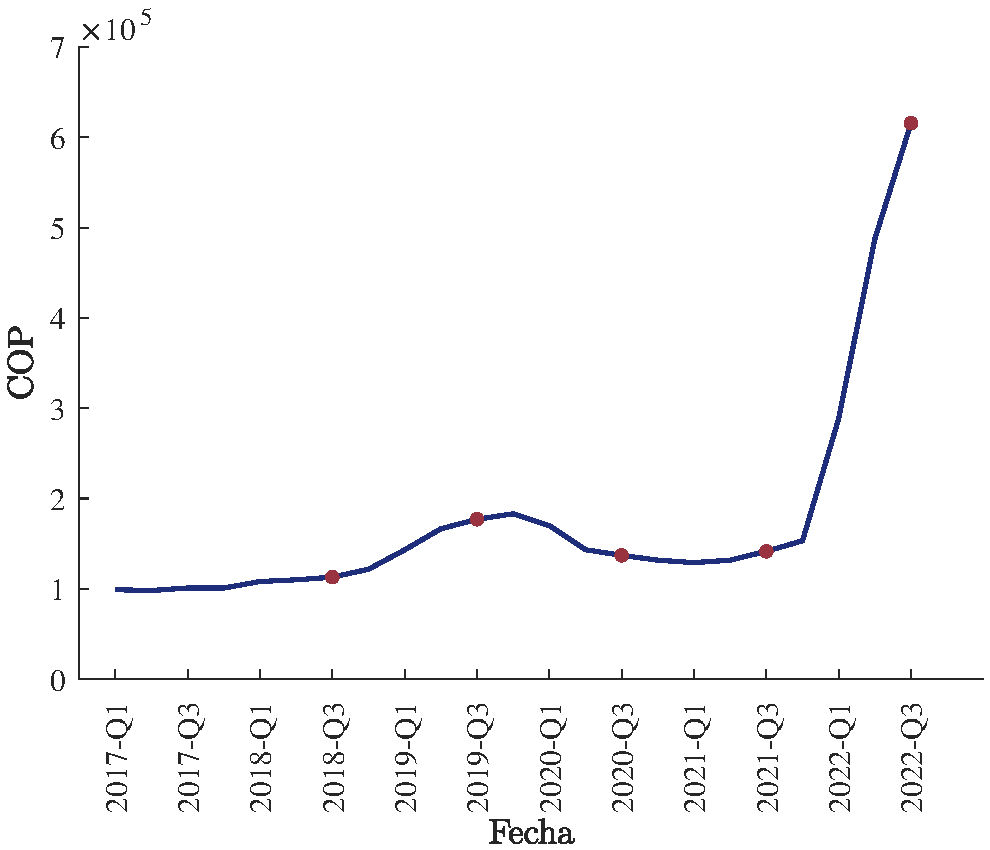
\includegraphics[width=0.8\textwidth]{Figures/Price_series.pdf}
    \end{figure}
\end{frame}

\begin{frame}{Precios Base Regalia}{Térmico}
    \begin{figure}
        \centering
        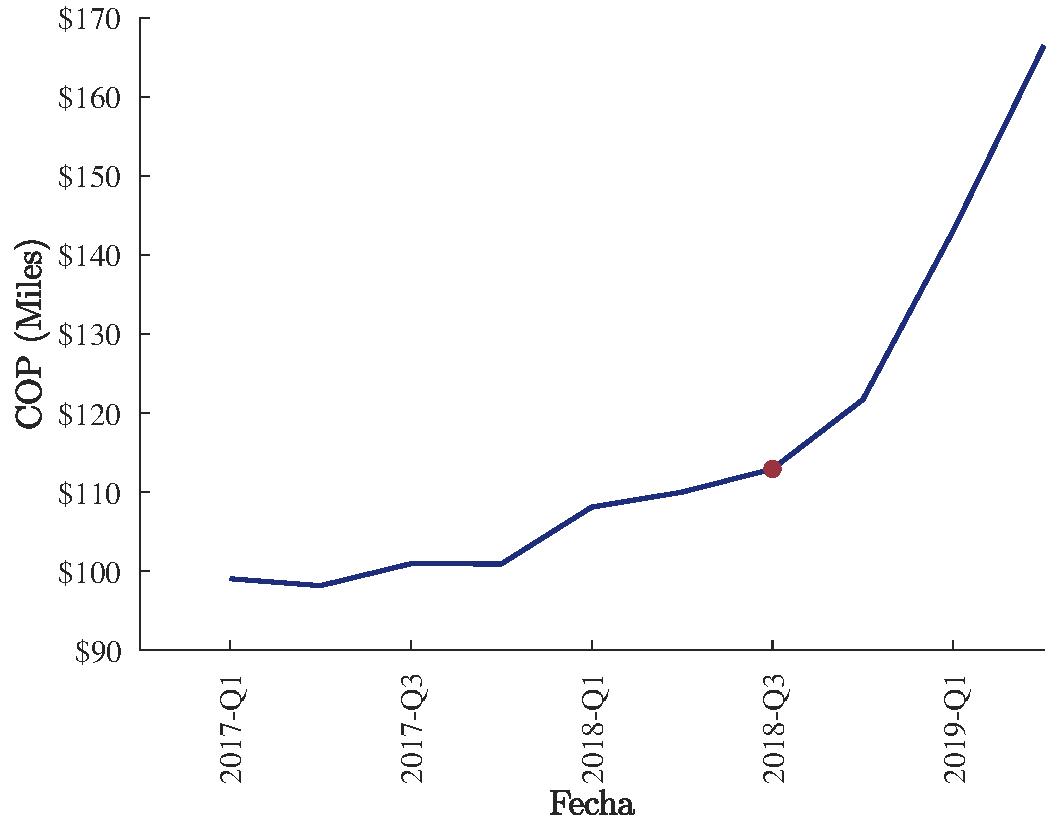
\includegraphics[width=0.8\textwidth]{Figures/oldCalc1.pdf}
    \end{figure}
\end{frame}

\begin{frame}{Precios Base Regalia}{Térmico}
    \begin{figure}
        \centering
        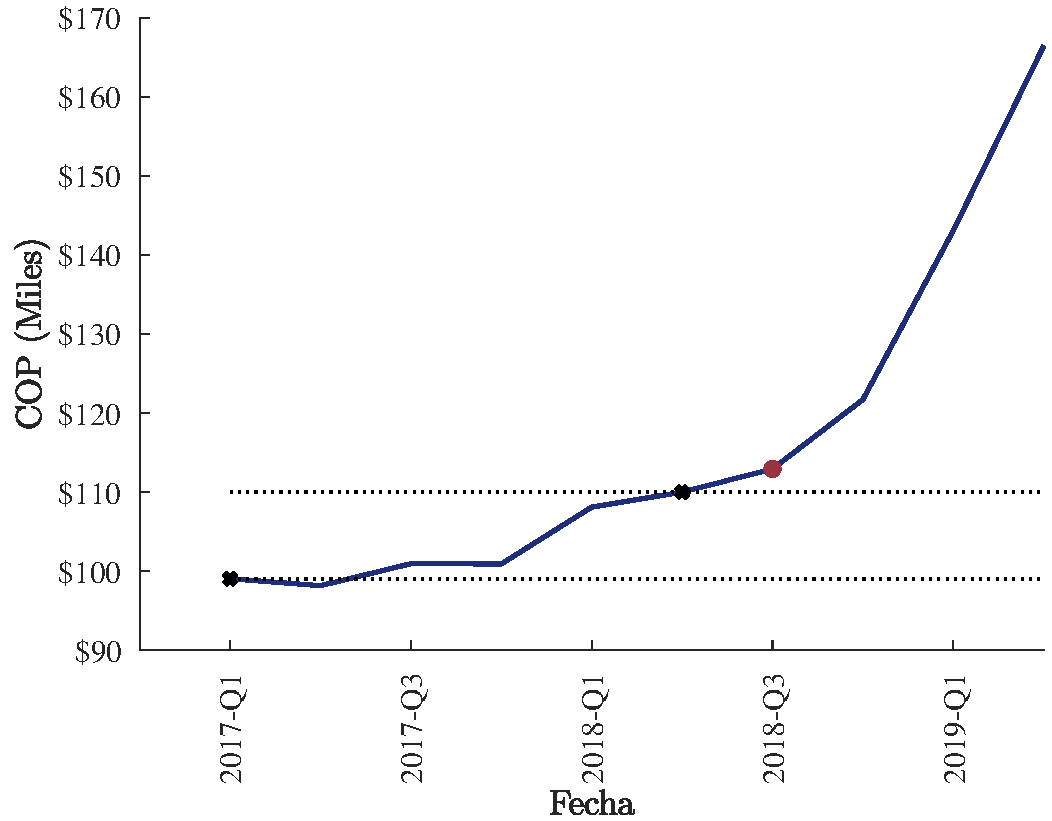
\includegraphics[width=0.8\textwidth]{Figures/oldCalc2.pdf}
    \end{figure}
\end{frame}

\begin{frame}{Precios Base Regalia}{Térmico}
    \begin{figure}
        \centering
        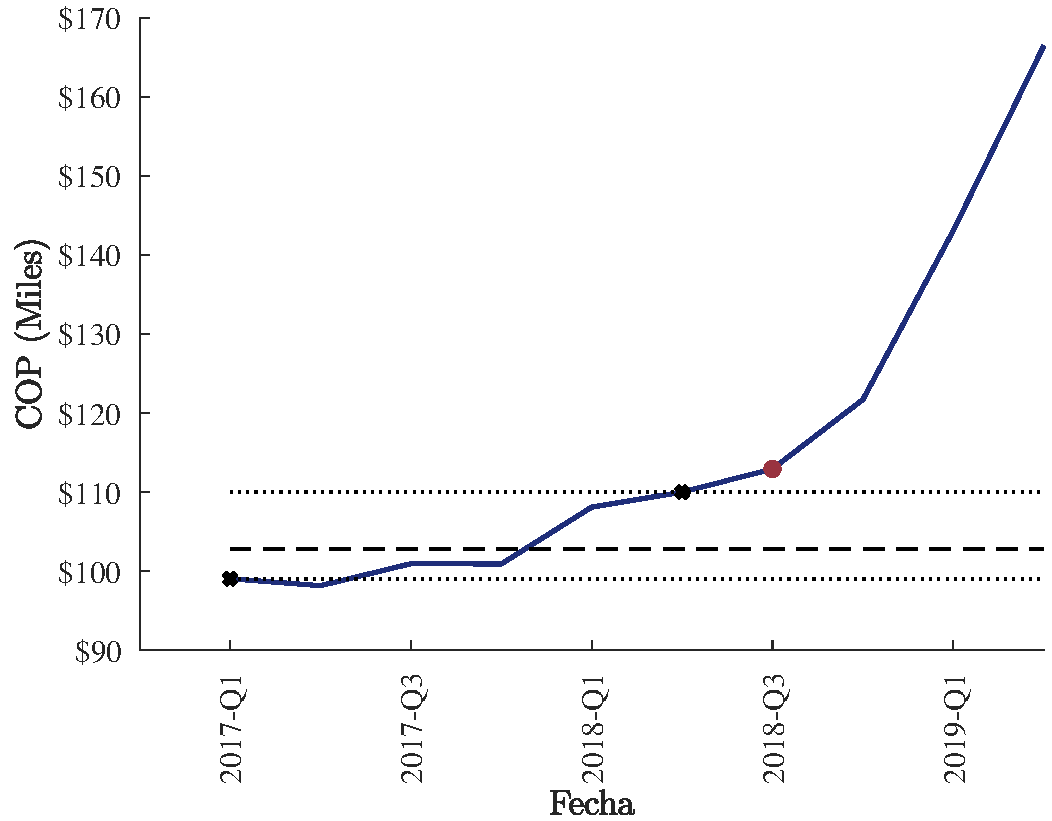
\includegraphics[width=0.8\textwidth]{Figures/oldCalc3.pdf}
    \end{figure}
\end{frame}

\begin{frame}{Precios Base Regalia}{Térmico}
    \begin{figure}
        \centering
        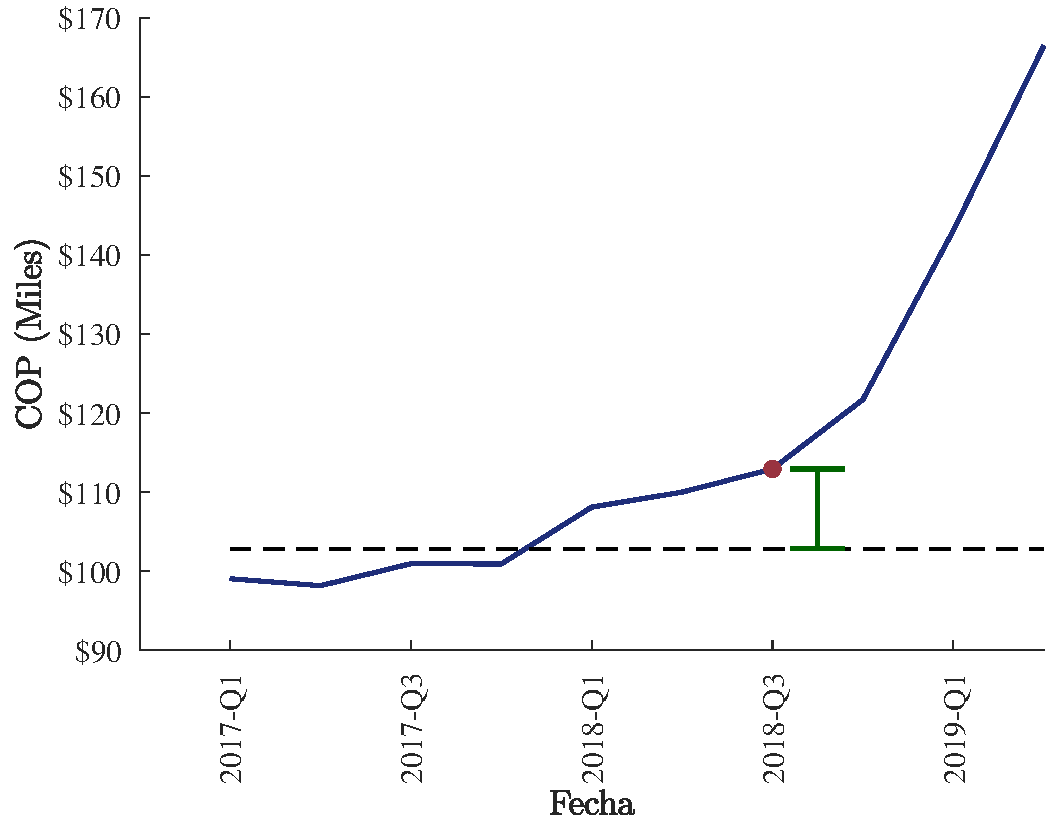
\includegraphics[width=0.8\textwidth]{Figures/oldCalc4.pdf}
    \end{figure}
\end{frame}

\begin{frame}{¿Qué concluimos?}
\begin{itemize}
    \item El cálculo actual es ciego a las tendencias de corto plazo de los precios. 
    \item Cuando los precios suben, la metodología actual sobre estima el porcentaje de la participación que le corresponde al contratista. 
    \item El año presente (2022) ha precensiado un aumento en precios agresivo. La metología actual penaliza la reciente alza en precios. 
\end{itemize}
\end{frame}

\begin{frame}{Mi propuesta}
\begin{itemize}
    \item Los precios son procesos Markovianos.
    \begin{enumerate}
        \item Tienen tendencias en el tiempo.
        \item Hay muchos estudios sobre la evolución de los precios en el tiempo. 
        \item Algunas referencias: \citet{Nag20}, \citet{Ryan73}. 
    \end{enumerate}
    \item Corrección de la metodología
    \begin{enumerate}
        \item Incorporar la tendencia de los precios en el corto plazo para calcular el porcentaje adicional que le corresponde al contratista. 
        \item Disminuye la varianza de la comisión. 
    \end{enumerate}
\end{itemize}
\end{frame}

\begin{frame}{Cálculo de la Participación}
    \begin{enumerate}
        \item Calcular la tendencia ($\nu$) de los precios en una ventana de 6 (seis) periodos anteriores al periodo de liquidación
        \begin{equation*}
            \nu = \frac{1}{5}\sum_{t=1}^5 P_{\ell-t}-P_{\ell-t-1}
        \end{equation*}
        donde $\ell$ es el periodo de liquidación y $P$ es el precio base del mineral.  
        \item Con base en la tendencia, el precio proyectado para el periodo de liquidación es
        \begin{equation*}
            \hat{P}_\ell = P_{\ell-6} + \nu\times6
        \end{equation*}
        \item El nuevo coeficiente es la razón entre el precio proyectado y el precio real
        \begin{equation*}
            \sfrac{P_\ell}{\hat{P}_\ell}
        \end{equation*}
    \end{enumerate}
\end{frame}

\begin{frame}{¿Cómo cambia el cálculo?}
    \begin{figure}
        \centering
        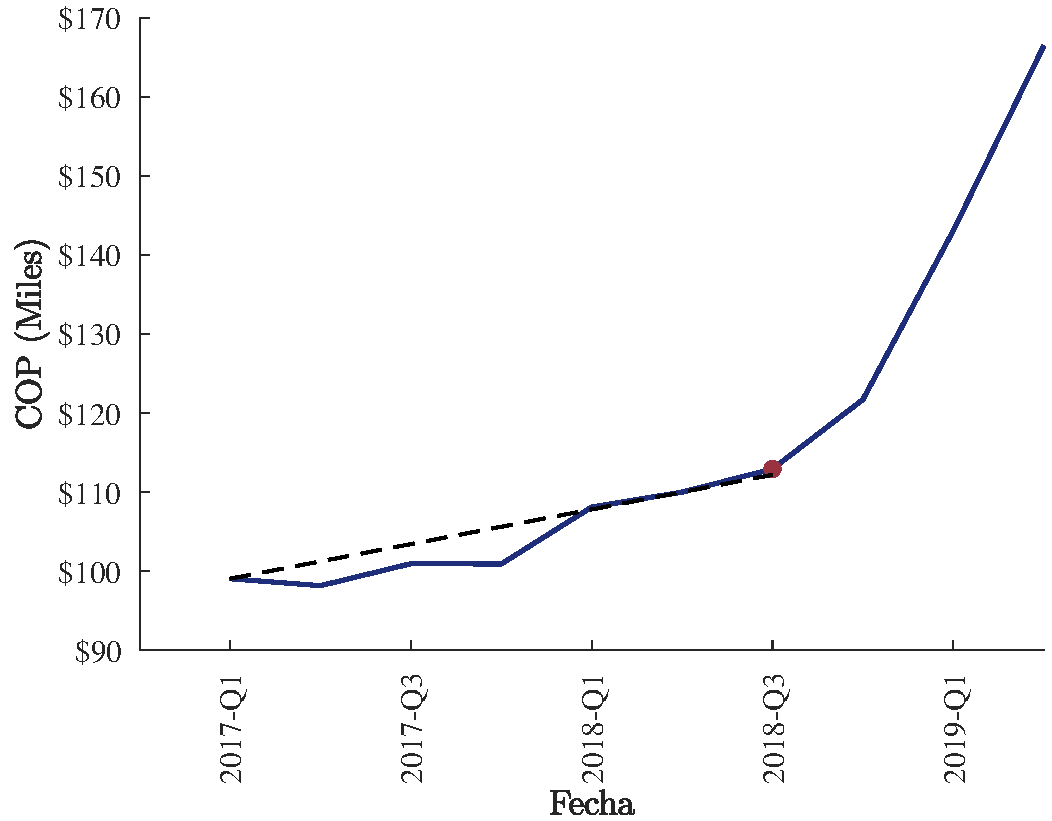
\includegraphics[width=0.8\textwidth]{Figures/newCalc.pdf}
    \end{figure}
\end{frame}

\begin{frame}{Relevancia para este año}
    \begin{figure}
        \centering
        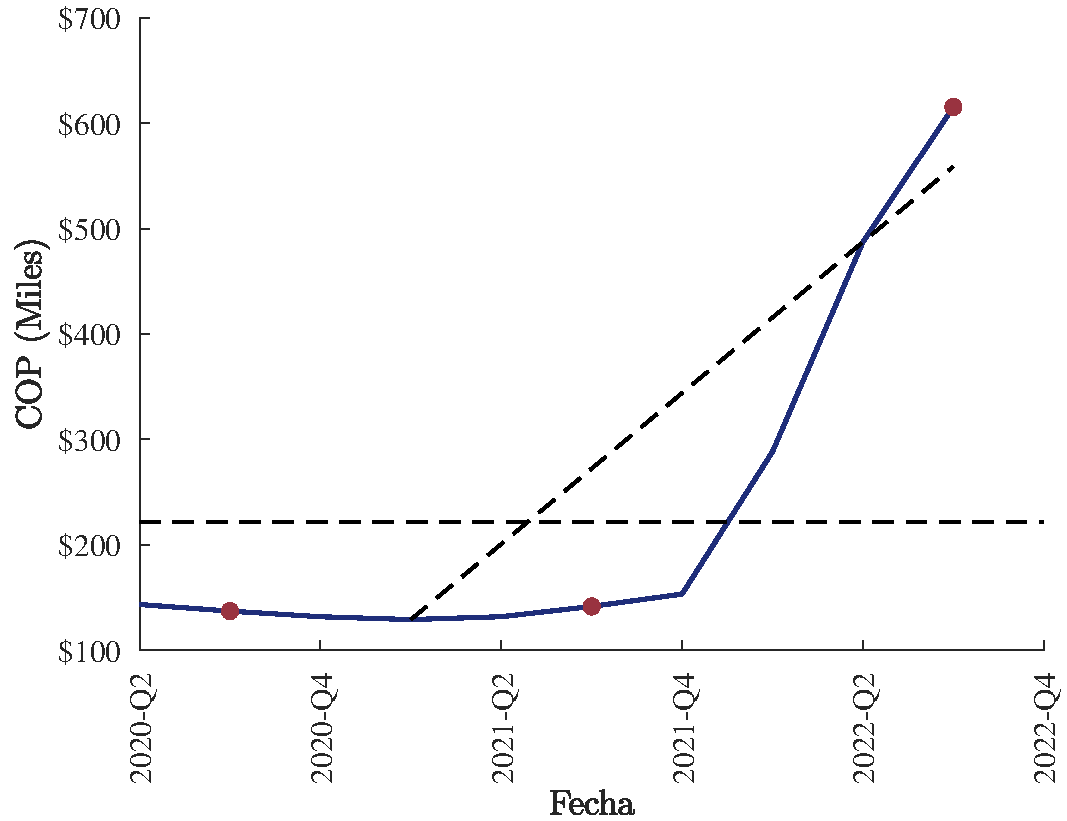
\includegraphics[width=0.8\textwidth]{Figures/newCalc2.pdf}
    \end{figure}
\end{frame}


\begin{frame}[allowframebreaks]{References}
    \bibliographystyle{apacite}
    \bibliography{references.bib}
\end{frame}

\end{document}

